\documentclass[a4paper,11pt]{article}
\input{/home/tof/Documents/Cozy/latex-include/preambule_doc.tex}
\input{/home/tof/Documents/Cozy/latex-include/preambule_commun.tex}
\newcommand{\showprof}{show them}  % comment this line if you don't want to see todo environment
\setlength{\fboxrule}{0.8pt}
\fancyhead[L]{\fbox{\Large{\textbf{VISIO}}}}
\fancyhead[C]{\textbf{Créer un salon de visioconférence}}
\newdate{madate}{10}{09}{2020}
\fancyhead[R]{\today} %\today
%\fancyhead[R]{Seconde - SNT}
\fancyfoot[L]{\vspace{1mm}Christophe Viroulaud}
\AtEndDocument{\label{lastpage}}
\fancyfoot[C]{\textbf{Page \thepage/\pageref{lastpage}}}
\fancyfoot[R]{\includegraphics[width=2cm,align=t]{/home/tof/Documents/Cozy/latex-include/cc.png}}

\begin{document}
\section{Se connecter: 2 méthodes}
\subsection{Avec mon identifiant ARENA (le plus simple)}
\begin{itemize}
    \item Se rendre \url{https://visio-lycees.education.fr}
    \item Choisir le guichet
    \item Entrer ses identifiants
\end{itemize}
\subsection{En créant un compte (pour voir toutes les applications existantes)}
\begin{itemize}
    \item Se rendre sur \url{https://apps.education.fr/}
    \item Cliquer \textbf{accéder à la plateforme}
    \item Choisir le guichet
    \item Cliquer sur \textbf{se connecter}
    \item Entrer l'adresse mail académique comme identifiant et créer un mot de passe
    \item Cliquer sur le premier lien: \textbf{Portail Apps}
\begin{center}
        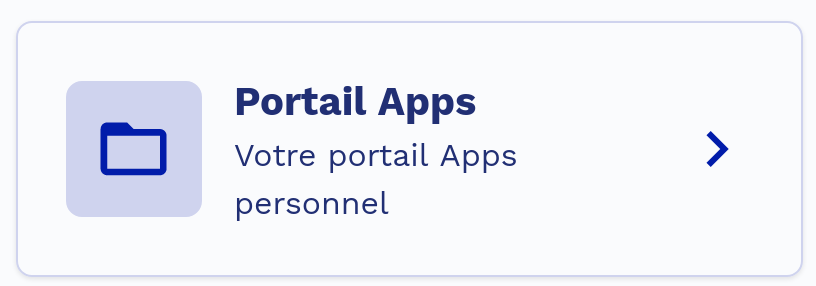
\includegraphics[width=5cm]{ressources/lien.png}
    
\end{center}    \item Aller dans le menu (en haut) \textbf{APPLICATIONS}
    \item Choisir \textbf{Visioconférence - BigBlueButton lycée}.
\end{itemize}
\section{Paramétrer un salon}
L'objectif est de créer un salon déjà configuré afin de n'avoir qu'à l'ouvrir le jour de la réunion.
\begin{itemize}
    \item Cliquer sur \textbf{Créer une salle de cours}
    \item Dans \textbf{Créer un cours}, renommer la salle. Ne pas cocher la case \textbf{salle d'attente}
    \item Dans \textbf{Gestion des permissions} effectuer les réglages suivants (figure \ref{reglages})
          \begin{center}
              \centering
              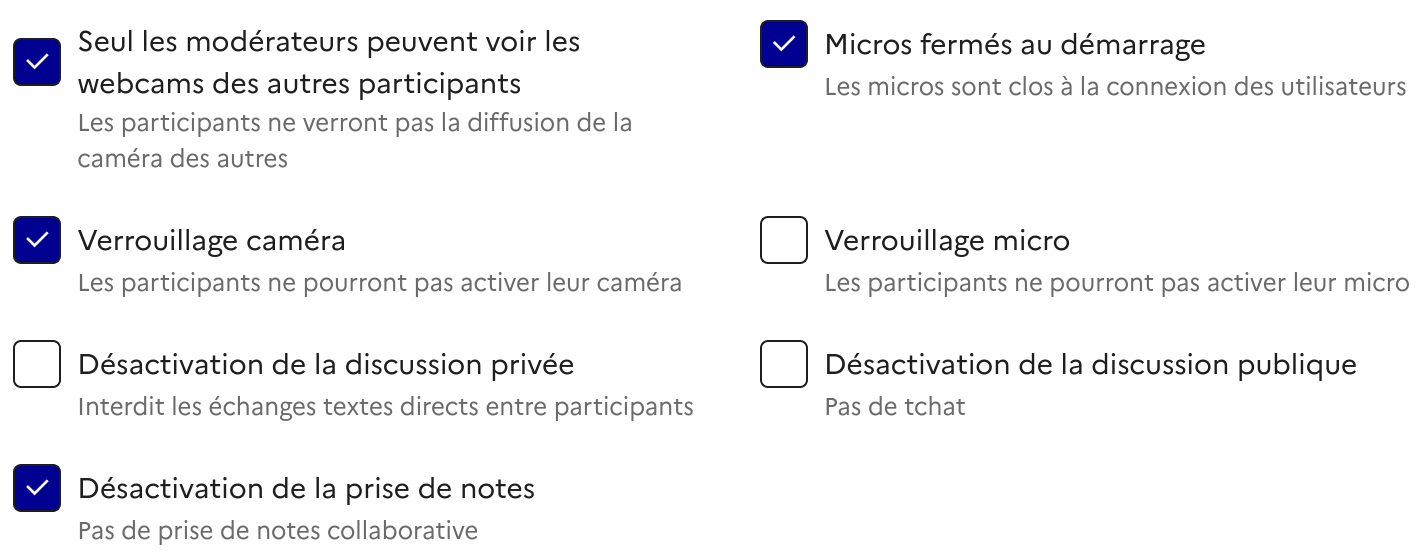
\includegraphics[width=11cm]{ressources/reglages.png}
              \captionof{figure}{Réglages}
              \label{reglages}
          \end{center}
    \item Enregistrer la configuration
\end{itemize}
\section{Tester le salon}
Pour se familiariser avec l'environnement et voir les derniers réglages possibles, il faut ouvrir le salon.
\begin{itemize}
    \item Cliquer \textbf{Lancer}.
    \item Cliquer sur le microphone pour qu'un test soit lancé (Il faut qu'un microphone soit présent sur la machine. Les ordinateurs portables en ont un intégré; il faut par contre en brancher un sur un poste fixe.)
    \item Autoriser l'utilisation du microphone par Firefox
    \item Les boutons en bas de l'écran permettent d'interagir avec les participants. Le bouton $\bigoplus$ permet par exemple de charger un pdf.
          \begin{center}
              \centering
              
\includegraphics[width=10cm]{ressources/boutons.png}
              \captionof{figure}{Interactions}
              \label{interagir}
          \end{center}
    Si la connexion est faible, l'affichage d'un diaporama peut influer sur la qualité de la visioconférence.
    
    \item Quelques réglages peuvent être effectués le jour de la présentation. Cliquer sur les trois points verticaux en haut à droite et choisir \textbf{ouvrir les paramètres} (figure \ref{reg2})
    \item \begin{center}
        \centering
        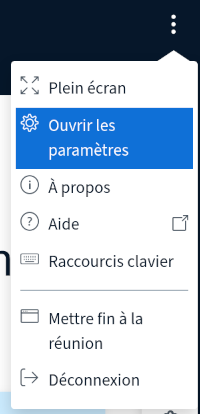
\includegraphics[width=3cm]{ressources/reglages2.png}
        \captionof{figure}{Options}
        \label{reg2}
    \end{center}
    
    \item Dans \textbf{Applications} cocher \textbf{Alertes Popup pour Nouveau participant}.
    \item Si la réunion connaît des problèmes de bande-passante il faudra tout décocher dans \textbf{Économies de données}.
\end{itemize}
\end{document}